\documentclass[12pt,addpoints]{evalua}
\grado{2$^\circ$ de Secundaria}
\cicloescolar{2023-2024}
\materia{Matemáticas 2}
\unidad{1}
\title{Examen de la Unidad}
\aprendizajes{
        \item Resuelve problemas de multiplicación y división con números enteros, fracciones y decimales positivos y negativos.
        \item Resuelve problemas de potencias con exponente entero y aproxima raíces cuadradas.
        \item Resuelve problemas de proporcionalidad directa e inversa y de reparto proporcional.
}
\author{Prof.: Julio César Melchor Pinto}
\begin{document}
\begin{questions}
      \question[10] Escribe sobre la línea el símbolo de mayor que ($>$), menor que ($<$), o igual ($=$) según corresponda.

      \begin{multicols}{2}
            \begin{parts}
                  % \part $\dfrac{2}{5}$ \fillin[$>$][0.5in] $\dfrac{1}{3}$\\[0.75em]
                  % \part $\dfrac{3}{4}$ \fillin[$<$][0.5in] $\dfrac{4}{5}$\\[0.75em]
                  % \part $\dfrac{2}{5}$ \fillin[$<$][0.5in] $\dfrac{2}{3}$\\[0.75em]
                  % \part $\dfrac{3}{2}$ \fillin[$=$][0.5in] $\dfrac{9}{6}$\\[0.75em]
                  % \part $\dfrac{5}{6}$ \fillin[$>$][0.5in] $\dfrac{4}{6}$\\[0.75em]
                  \part $\dfrac{4}{3}$ \fillin[$>$][0.5in] $\dfrac{5}{4}$\\[0.75em]
                  \part $\dfrac{1}{3}$ \fillin[$=$][0.5in] $\dfrac{9}{3}$\\[0.75em]
                  \part $\dfrac{2}{3}$ \fillin[$<$][0.5in] $\dfrac{3}{2}$\\[0.75em]
                  \part $\dfrac{3}{4}$ \fillin[$>$][0.5in] $\dfrac{2}{3}$\\[0.75em]
                  \part $\dfrac{5}{6}$ \fillin[$>$][0.5in] $\dfrac{4}{5}$\\[0.75em]
                  % \part $-51$ \fillin[$>$][0.5in] $-55$\\[0.75em]
                  % \part $-77$ \fillin[$>$][0.5in] $-177$\\[0.75em]
                  % \part $-100$ \fillin[$<$][0.5in] $-99$\\[0.75em]
                  % \part $-182$ \fillin[$>$][0.5in] $-189$\\[0.75em]
                  % \part $-97$ \fillin[$<$][0.5in] $-96.2$\\[0.75em]
                  \part $-36$ \fillin[$>$][0.5in] $-39$\\[0.75em]
                  \part $-3.5$ \fillin[$<$][0.5in] $-2.2$\\[0.75em]
                  \part $-12$ \fillin[$<$][0.5in] $-11$\\[0.75em]
                  \part $-10.001$ \fillin[$>$][0.5in] $-100.01$\\[0.75em]
                  \part $-0.99$ \fillin[$>$][0.5in] $1.01$\\[0.75em]
            \end{parts}
      \end{multicols}

      \newpage

      \question[20] Realiza las operaciones con exponentes indicadas en cada uno de los siguientes incisos.

      \begin{multicols}{2}
            \begin{parts}
                  \part $x^2y^3z^4 \cdot x^5z^4=$
                  \begin{solutionbox}{2cm}
                        $x^2y^3z^4 \cdot x^5z^4 = x^7y^3z^8$
                  \end{solutionbox}

                  % \part $x^3x^2x^3=$
                  % \begin{solutionbox}{2cm}
                  %       $x^3x^2x^3 = x^8$
                  % \end{solutionbox}

                  \part $7x^2\cdot 3x^4 \cdot 6x^2=$
                  \begin{solutionbox}{2cm}
                        $7x^2\cdot 3x^4 \cdot 6x^2 = 126x^8$
                  \end{solutionbox}

                  % \part $(-4x^2)(-5x^3)=$
                  % \begin{solutionbox}{2cm}
                  %       $(-4x^2)(-5x^3) = 20x^5$
                  % \end{solutionbox}

                  % \part $(-8x)(-5x^5)=$
                  % \begin{solutionbox}{2cm}
                  %       $(-8x)(-5x^5) = 40x^6$
                  % \end{solutionbox}

                  \part $(-x^4)(2y^3)=$
                  \begin{solutionbox}{2cm}
                        $(-x^4)(2y^3) = -2x^4y^3$
                  \end{solutionbox}

                  % \part $(-5a^4)(-3a^2)=$
                  % \begin{solutionbox}{2cm}
                  %       $(-5a^4)(-3a^2) = 15a^6$
                  % \end{solutionbox}

                  \part  $x^3\cdot x^5\cdot x=$
                  \begin{solutionbox}{2cm}
                        $x^3\cdot x^5\cdot x = x^9$
                  \end{solutionbox}

                  % \part $(-3a^4)(8a^2)=$
                  % \begin{solutionbox}{2cm}
                  %       $(-3a^4)(8a^2) = -24a^6$
                  % \end{solutionbox}

                  \part $4x^2\cdot x^5\cdot 5x^8=$
                  \begin{solutionbox}{2cm}
                        $4x^2\cdot x^5\cdot 5x^8 = 20x^{15}$
                  \end{solutionbox}

                  \part $\dfrac{x^{13}y^{18}z^4}{x^{11}y^9z^4}=$
                  \begin{solutionbox}{2cm}
                        $\dfrac{x^{13}y^{18}z^4}{x^{11}y^9z^4} = x^2y^9$
                  \end{solutionbox}

                  \part $\dfrac{81a^5b^{12}c^9}{9a^3b^{7}c^5}=$
                  \begin{solutionbox}{2cm}
                        $\dfrac{81a^5b^{12}c^9}{9a^3b^{7}c^5} = 9a^2b^5c^4$
                  \end{solutionbox}

                  \part $\dfrac{x^{4}y^{12}z^{13}}{x^{3}y^{12}z^{13}}=$
                  \begin{solutionbox}{2cm}
                        $\dfrac{x^{4}y^{12}z^{13}}{x^{3}y^{12}z^{13}} = x$
                  \end{solutionbox}

                  % \part $\left(a^3 b^5 c^{11} \right)^7=$
                  % \begin{solutionbox}{2cm}
                  %       $\left(a^3 b^5 c^{11} \right)^7 = a^{21}b^{35}c^{77}$
                  % \end{solutionbox}

                  \part $\left(x^4 y^5\right)^6=$
                  \begin{solutionbox}{2cm}
                        $\left(x^4 y^5\right)^6 = x^{24}y^{30}$
                  \end{solutionbox}

                  \part $\left(a^4b^4c^5d^{11}\right)^9=$
                  \begin{solutionbox}{2cm}
                        $\left(a^4b^4c^5d^{11}\right)^9 = a^{36}b^{36}c^{45}d^{99}$
                  \end{solutionbox}

            \end{parts}
      \end{multicols}

      \newpage
      \question[10] Escribe el número que representa el punto indicado en la recta numérica de cada uno de los siguientes incisos.
      \begin{multicols}{2}
            \begin{parts}
                  \part 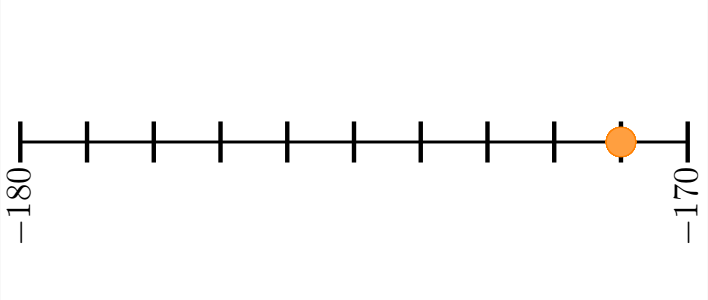
\includegraphics[width=140px]{../images/recta_num_-171.png} \\[-0.5em]   \fillin[$-171$][1.5in]
                  \part 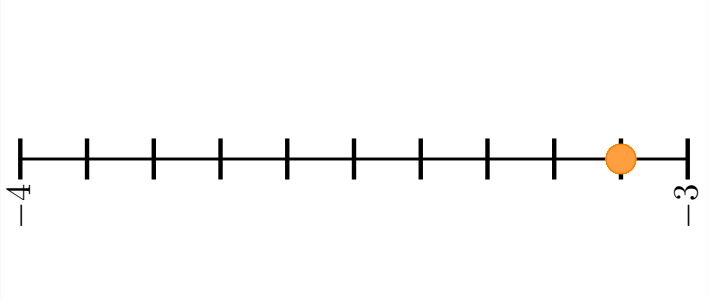
\includegraphics[width=140px]{../images/recta_num_-3.1.png} \\[-0.5em]   \fillin[$-3.1$][1.5in]
                  \part 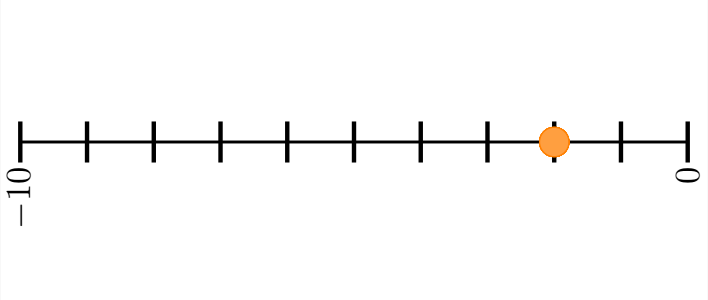
\includegraphics[width=140px]{../images/recta_num_-2.png}   \\[-0.5em] \fillin[$-2$][1.5in]
                  \part 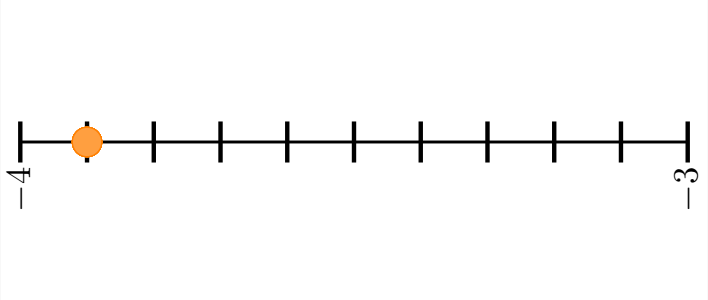
\includegraphics[width=140px]{../images/recta_num_-3.9.png} \\[-0.5em]   \fillin[$-3.9$][1.5in]
                  \part 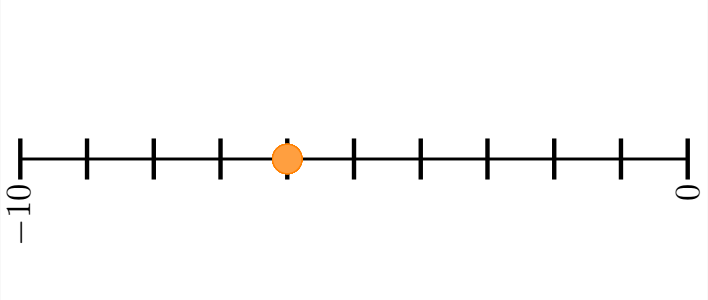
\includegraphics[width=140px]{../images/recta_num_-6.png}   \\[-0.5em] \fillin[$-6$][1.5in]
                  \part 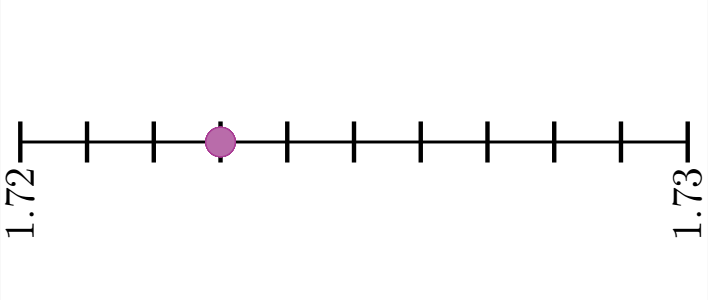
\includegraphics[width=140px]{../images/recta_num_1.723.png}\\[-0.5em]  \fillin[$1.723$][1.5in]
                  \part 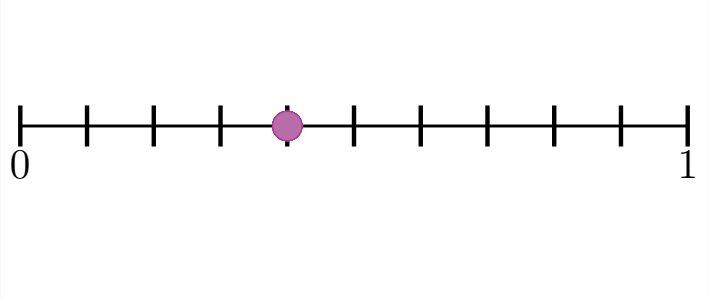
\includegraphics[width=140px]{../images/recta_num_0.4.png}  \\[-0.5em]  \fillin[$0.4.$][1.5in]
                  \part 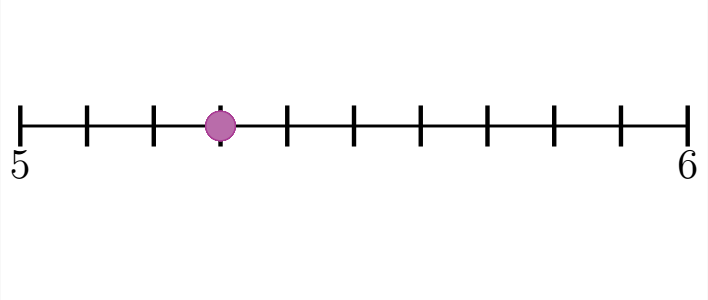
\includegraphics[width=140px]{../images/recta_num_5.3.png}  \\[-0.5em]  \fillin[$5.3.$][1.5in]
                  \part 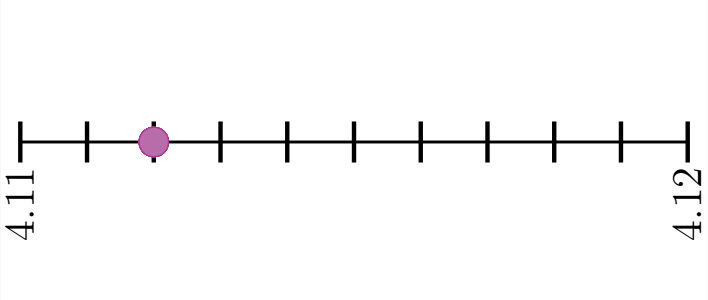
\includegraphics[width=140px]{../images/recta_num_4.112.png}\\[-0.5em]  \fillin[$4.11$][1.5in]
                  \part 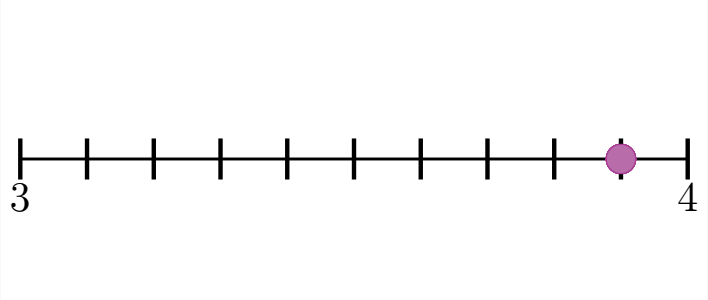
\includegraphics[width=140px]{../images/recta_num_3.9.png}  \\[-0.5em]  \fillin[$3.9.$][1.5in]
                  % \part 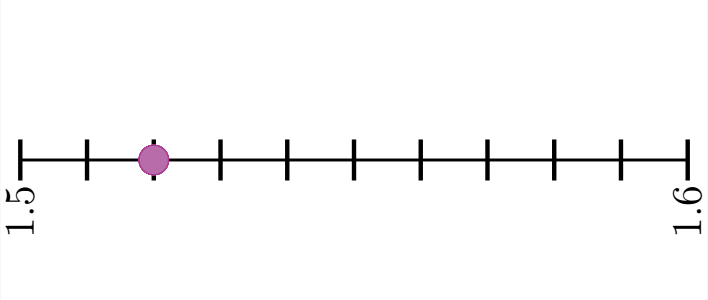
\includegraphics[width=150px]{../images/recta_num_1.52.png} \\[-0.5em] \fillin[$1.52$][1.5in]   \\[-1.4em]
                  % \part 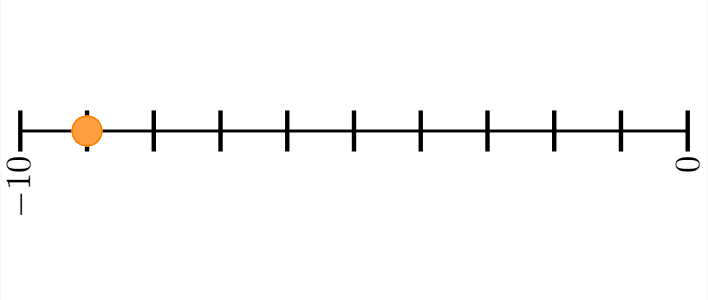
\includegraphics[width=150px]{../images/recta_num_-9.png}   \\[-0.5em] \fillin[$-9$][1.5in]     \\[-1.4em]
                  % \part 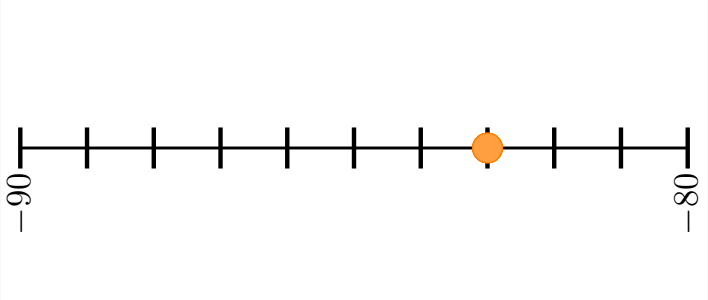
\includegraphics[width=150px]{../images/recta_num_-83.png}  \\[-0.5em]  \fillin[$-83$][1.5in]   \\[-1.4em]
                  % \part 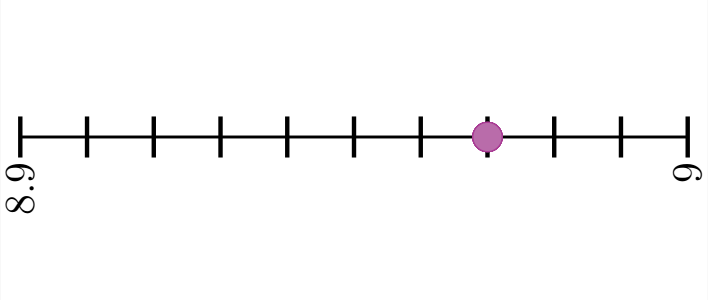
\includegraphics[width=150px]{../images/recta_num_8.97.png} \\[-0.5em]  \fillin[$8.97$][1.5in]  \\[-1.4em]
                  % \part 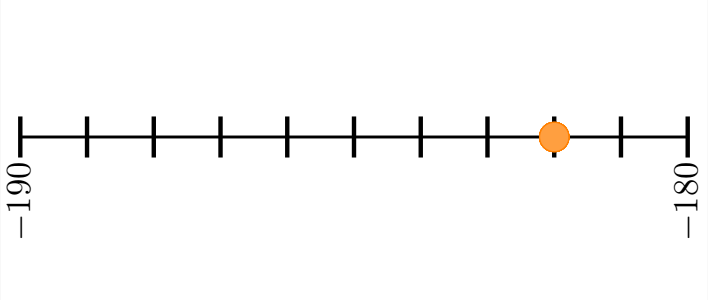
\includegraphics[width=150px]{../images/recta_num_-182.png} \\[-0.5em]   \fillin[$-182$][1.5in] \\[-1.4em]
                  % \part 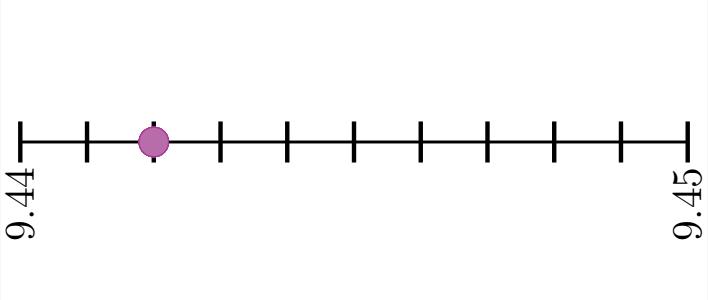
\includegraphics[width=150px]{../images/recta_num_9.442.png}\\[-0.5em]  \fillin[$9.44$][1.5in]  \\[-1.4em]
                  % \part 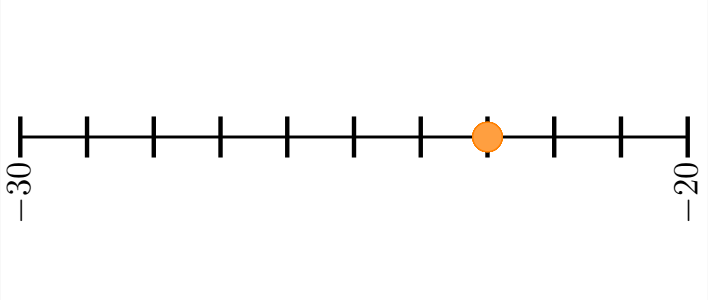
\includegraphics[width=150px]{../images/recta_num_-23.png}  \\[-0.5em]  \fillin[$-23$][1.5in]   \\[-1.4em]
                  % \part 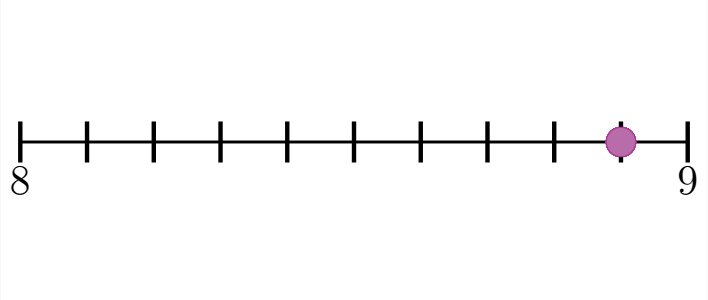
\includegraphics[width=150px]{../images/recta_num_8.9.png}  \\[-0.5em]  \fillin[$8.9$][1.5in]   \\[-1.4em]
                  % \part 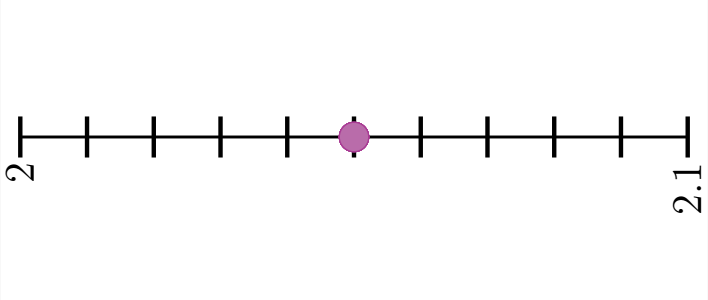
\includegraphics[width=150px]{../images/recta_num_2.05.png} \\[-0.5em]  \fillin[$2.05$][1.5in]  \\[-1.4em]
                  % \part 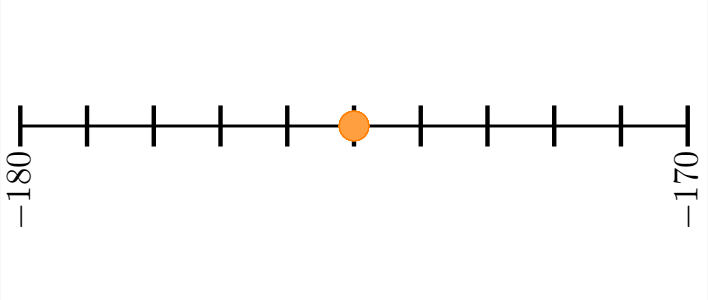
\includegraphics[width=150px]{../images/recta_num_-175.png} \\[-0.5em]   \fillin[$-175$][1.5in]
            \end{parts}
      \end{multicols}
\end{questions}
\end{document}